
\section{대략적인 복잡도 분석}


해당절과 다음절의 복잡도 분석은 quicksort에 모든 입력값에 중복값이 존재 하지않음을 미리 가정하고있다.

\subsection{최악의 분할 케이스} 

최악의 경우 분할 케이스를 생각해보자 
이는 왼쪽 오른쪽 분할이 한쪽으로 쏠려(오름차순,내림차순) 극도로 불균형하게 일어났을때이다.
피봇값에 의한 분할이 아예 일어나지 않을 때 최악의 케이스가 된다.
이때 비용을 나타낸 재귀함수다.
$$T(n) = T(n-1) + cn $$
\begin{align*}
    T(n) &= T(n-1) + cn \\
    &= T(n-2) + c(n-1) +cn \\
    &= c\sum^{n}_{k=1}k \\
    &= \dfrac{1}{2} cn^{2}\\
    &= \Theta (n^{2})    
\end{align*}


따라서 시간복잡도는 $\Theta(n^2)$이다.

\subsection{최선의 분할 케이스} 

정확하게 반으로 나누어 졌을때 최선의 분할 케이스이다.

이때의 비용을 나타낸 재귀함수는
$$T(n) = 2T(\dfrac{n}{2}) + cn$$
이다.

\begin{figure}[h!]
    \centering
    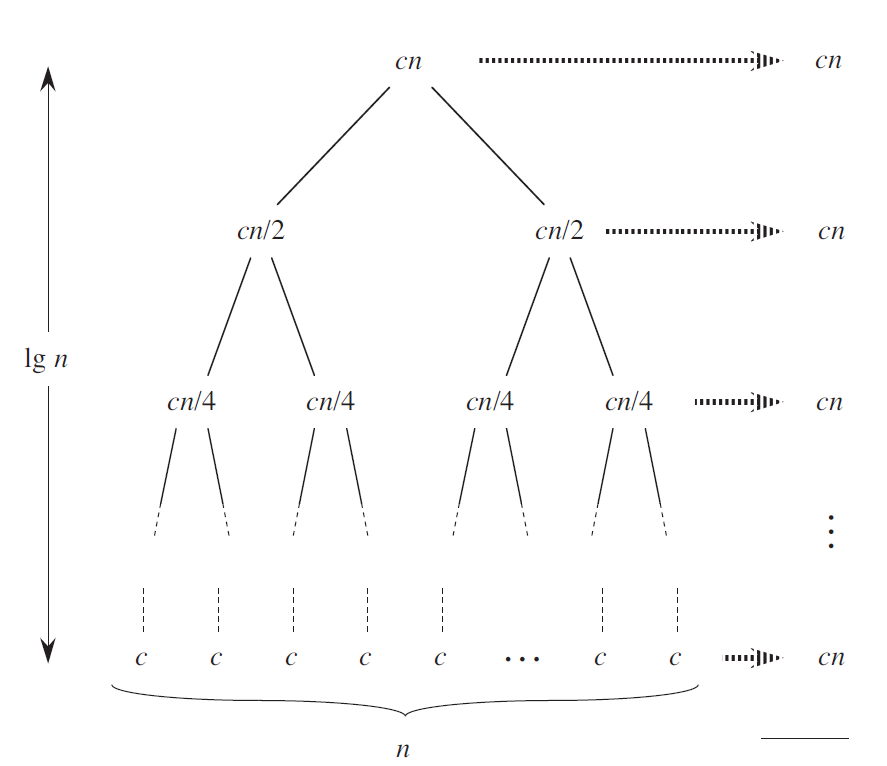
\includegraphics[scale=0.5]{./QuickSort/pic/q2.png}
    \caption{quick sort 최선의 분할 케이스 재귀 트리\cite{reference1}}
\end{figure}
그림 2의 재귀트리를 통해서 전체 비용을 계산하여 시간복잡도를 구하면 $\Theta(n \lg n)$이다. \footnote{marster theory를 사용하여 바로 구해도 된다.}

\subsection{일반적인 케이스 직관적인 방법} 
평균적인 경우로 생각해볼수있는 다음 두가지 경우에 대해서 논의를 해 볼 것이다.
\begin{itemize}
    \item 항상 9:1로 분할하는 경우
    \item 최악의 경우와 최선의 경우가 번갈아 나타나는 경우
\end{itemize}

\subsubsection{항상 9:1로 분할하는 경우}

\begin{figure}[h!]
    %\centering
    \raggedleft
    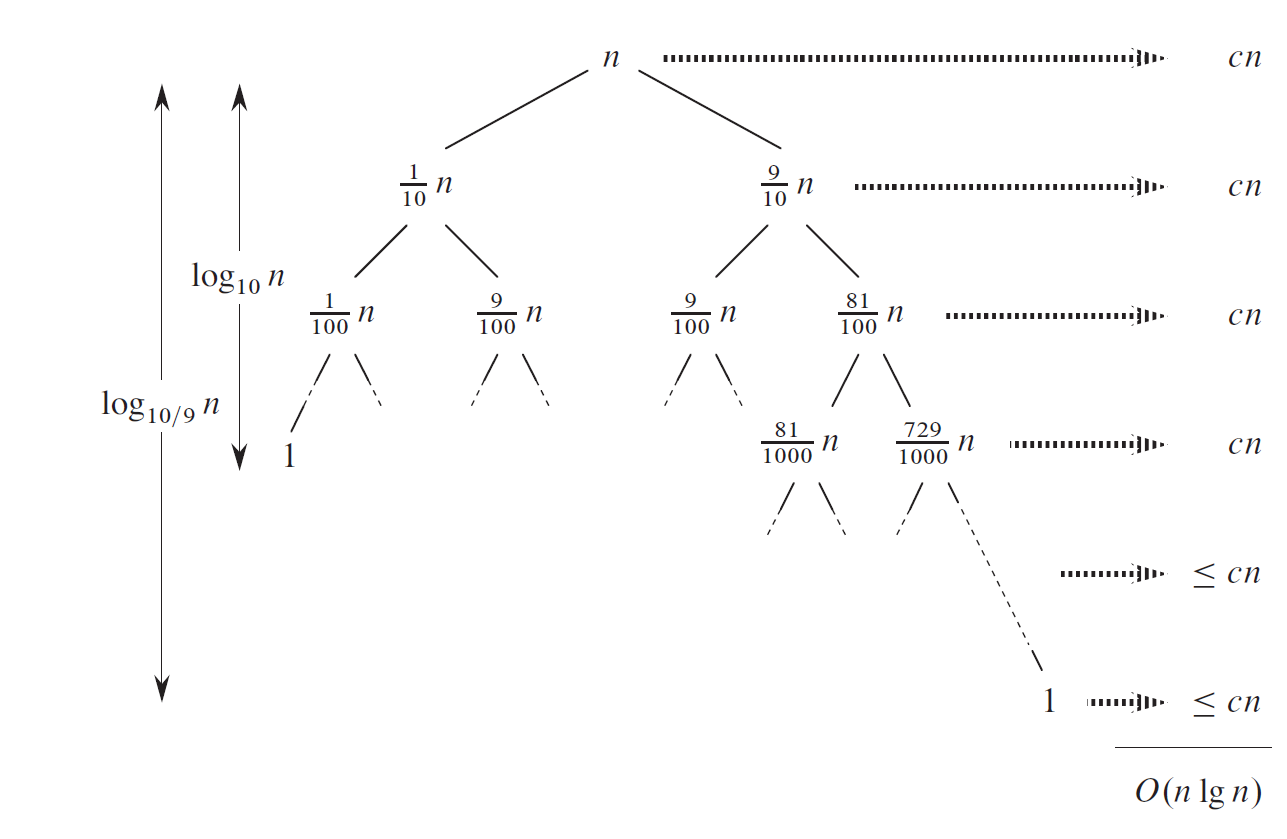
\includegraphics[scale=0.4]{./QuickSort/pic/q9.png}
    \caption{9:1로 분할하는 재귀 트리\cite{reference1}}
\end{figure}
다음의 경우 재귀 함수는 다음이 성립한다.
$$T(n) \le T\left(\dfrac{9n}{10}\right) + T\left(\dfrac{n}{10}\right)+ cn$$


이다. 
이때 재귀트리는 깊이 $\log_{10}n$까지 각 깊이의 비용이 $cn$이고 그 밑 부터는 $cn$보다 작은 비용이 든다 따라서 깊이 $\log_{10/9}n$에 각 깊이 비용 $cn$인것보다 비용이 작으므로 $n\log_{10/9}n = O(n \log n)$이 된다. 따라서 $T(n) = \Theta(n \log n)$


\subsubsection{최악의 경우와 최선의 경우가 번갈아 나타나는 경우}

\begin{figure}[h!]
    \centering
    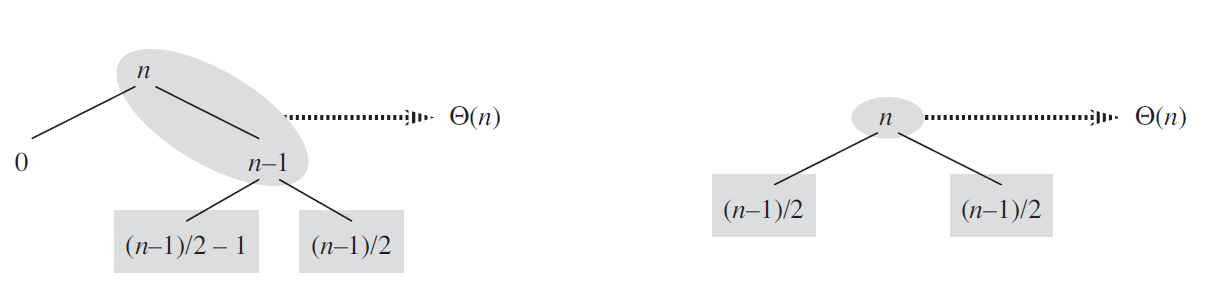
\includegraphics[scale=0.5]{./QuickSort/pic/q3.png}
    \caption{최악,최선이 번갈아 나타나는 재귀 트리\cite{reference1}}
\end{figure}

T(n) 일때의 시간복잡도와 T(n-1)일때의 시간복잡도는 둘다 $\Theta(n)$이다. 따라서 이 둘의 시간복잡도를 합쳐도 결국 $\Theta(n)$이고 이를 합쳐서 보면 결국에 최선의 분할 케이스가 된다 따라서 이때의 시간복잡도는 결국 $\Theta(n \lg n)$이다.
